\newpage

\section{Introduction}
Low birth weight (LBW) is defined by the World Health Organisation as a birth of an infant weighing less than 2500 grams. Low birth weight is closely associated with fetal and perinatal mortality, inhibited growth and cognitive development, and chronic diseases later in life. Physicians are therefore interested in understanding the effects of different behavioural and environmental variables on the likelihood of having a low birth weight.

The variables identified in \hyperlink{tab:variables}{Table 1} have been shown to be associated with low birth weight in the obstetrical literature. The goal of this study is to ascertain if these variables were important in the population being served in the medical center where this data were collected. We then build, compare, and discuss different models for predicting the likelihood of a low weight birth given these variables. 

\vspace{0.5cm}
\renewcommand{\arraystretch}{1.5}
\begin{table}[ht]
    \centering
    \begin{tabular}{ l|l } 
     \hline \hline
      \textbf{Variable} & \textbf{Abbreviation} \\
      \hline
     Low Birth Weight (0 or 1) & LOW \\
     \hline
     Age of the Mother in Years & AGE \\
     \hline
     Weight in pounds at the last menstrual period & LWT \\
     \hline
     Race (1 - White, 2 = Black, 3 = Other) & RACE \\
     \hline
     Smoking status during pregnancy (Yes = 1, No = 0) & SMOKE \\
     \hline
     Number of previous premature labours & PTL \\
     \hline
     History of hypertension & HT \\
     \hline
     Presence of uterine irritability & UI \\
     \hline
     Number of visits to physician during first trimester & FTV \\
     \hline
     Birth weight in grams & BWT \\
     \hline \hline
    \end{tabular}
    \caption{Variables included in the dataset.}
    \label{tab:variables}
\end{table}
\vspace{0.5cm}

\section*{Review of the Obstetrical Literature}
Reviewing the obstetrical literature allows us to understand how these variables and their interactions should influence the likelihood of a low birth weight. This information can then be compared with the results from an exploratory analysis of the data, allowing us to determine how our data differs from what would be expected and to make informed decisions when building predictive models.

\subsection{Effects of variables on low birth weight}
A brief description of the effect of each variable on low birth weight is given below.
\begin{itemize}
    \item \textbf{AGE:} Fraser and Brockert [1995] showed that teenage mothers have a significantly higher risk than mothers who were 20 to 24 years of age of delivering an infant who had low birth weight.\cite{AgeYoung} However, advancing maternal age is associated with a decreased potential for fetal growth and it has been shown that the adjusted risk for low birth weight at term is the lowest in younger mothers and increases with advancing maternal age.\cite{MaternalAge}
    
    \item \textbf{SMOKE:}
    Smoking during pregnancy inhibits full fetal development and is closely associated with low birth weight.\cite{SmokeLBW} However, the degree to which smoking affects low birth weight varies significantly with the average number of cigarettes smoked per day, with birth weight decreasing as the category of cigarette number per day increases.\cite{SmokeReduction} This study uses a binary SMOKE variable - a more detailed categorisation of smokers would most likely improve the quality of the models.
    
    \item \textbf{RACE:}
    There is a higher rate of LBW among black women when compared with white women.\cite{RaceDifference} Race effectively acts as a proxy variable - encoding information about sociodemographic, health-related, and behavioural differences between different racial groups.\cite{RaceLBW}
    
    \item \textbf{LWT:}
    Progressive increase in pre-pregnancy weight was paralleled by progressive increase in mean birth weight and decrease in the incidence of low weight births.\cite{Weight}
    
    \item \textbf{PTL:}
    The risk of the birth of a subsequent low birthweight infant is 2 to 5 times higher than average for mothers who have had a previous low birthweight delivery and increases with the number of prior low-weight births.\cite{bakketeig1979tendency}
    
    \item \textbf{HT:}
    Both chronic and pregnancy induced hypertension are strongly associated with retarded fetal growth and pre-term birth. As a result, maternal hypertension is strongly associated with low infant birthweight. \cite{InducedHT}\cite{HTRace}
    
    \item \textbf{FTV:}
    Increasing the number of physician visits can lead to earlier and more accurate diagnosis of LBW risk factors. Many studies have established a link between date of the first visit, total number of visits and length of pregnancy and LBW, a relation that is stronger if the first visit is delayed or if the number of visits is smaller than normal.\cite{FTV1}\cite{FTV2}\cite{FTV3}
    
    \item \textbf{UI:}
    The incidence of preterm labour in women with uterine irritability is not as frequent as in patients with other high-risk factors. However, preterm labour does occur in patients with uterine irritability at a rate higher than that in the general obstetric population.\cite{UI}
    
    
\end{itemize}

\subsection{Interactions between variables}
An interaction describes a situation in which the effect of one non-dependent variable on 'LOW' is dependant on the state of a second non-dependent variable. This is equivalent to saying the effects of the the non-dependent variables are not additive. Listed below are the interactions which are most relevant according to the obstetrical literature.

\begin{itemize}
    \item \textbf{SMOKE/AGE -}
    Older mothers, who are already at risk of giving birth to low birthweight infants, might be more susceptible to the effects of maternal smoking. [reference] determined that maternal age has a modifying effect on the association between maternal smoking and birthweight. The association between low birthweight and age increases with maternal age.\cite{SmokeAge}
    
    \item \textbf{SMOKE/RACE -}
    The LBW risk difference associated with smoking is greater among black women. This might be due to the fact that even if black women smoked significantly fewer cigarettes per day, they might have higher cotinine levels compared to white women. \cite{SmokeRace}
    
    \item \textbf{AGE/FTV -}
    For adult first-time mothers, fewer than 10 prenatal care visits was the only significant factor affecting LBW. Therefore, health education programs or prenatal care aimed at preventing LBW should be tailored according to the age of pregnant mothers. The effect of FTV on LBW is stronger for younger mothers.\cite{AgeFTV}
    
    \item \textbf{UI/PTL -}
    
    
\end{itemize}

\section{Structure of the Dataset}
A total of 189 subjects took part in the study. There are no missing data. In this study, there is a single binary response variable "LOW", where

\begin{equation}
    \text{LOW}=
    \begin{cases}
      1, & \text{if}\ \text{Birth weight} < 2500\text{g} \\
      0, & \text{otherwise}
    \end{cases}
\end{equation}

There are three continuous predictor variables (AGE, LWT, FTV), and five categorical predictor variables (RACE, SMOKE, PTL, HT, and UI).

\section{Exploratory Analysis}
An exploratory analysis is performed, first investigating the correlation between the predictor variables and the response variable, and then checking for meaningful interactions between predictor variables. The reasons for these analyses are twofold:
\begin{itemize}
    \item Investigate whether the associations and correlations in our data are consistent with the obstetrical literature.
    \item As a guideline for which main effects and interactions should be included in the candidate models.
\end{itemize}

Note that when we calculate correlation, we're not making any inferences about causality. We are instead using it to compare the associations in our data with those in the obstetrical literature to see if our data is consistent. Also a significant correlation with low birthweight gives us reason to strongly consider these variables as main effects in our candidate models.

\subsection{Correlation with LBW}
The Spearman correlation coefficient was calculated between the dependant variable (BWT) and each of the continuous variables - AGE, LTW, FTV, and PTL. The Spearman correlation was chosen due to the non-normal distribution of each of these variables, as determined by a series of Shapiro-Wilks tests. The Spearman correlation coefficients and related p-values are given in \hyperlink{tab:Spearman}{Table 2}. Both LWT and PTL are significantly correlated with BWT, with p-values of 0.001 and 0.005 respectively. They are therefore strong candidates to consider as parameters in our candidate models.

\newpage
\renewcommand{\arraystretch}{1.5}
\begin{table}[!htb]
    \centering
    \begin{tabular}{ |c|c|c|c|c| } 
     \hline
     & AGE & LWT & FTV & PTL \\
     \hline
     $\rho$ & 0.061 & 0.248 & 0.07 & -0.204 \\
     \hline
     p-value & 0.404 & \cellcolor{blue!25}0.001 & 0.338 & \cellcolor{blue!25}0.005 \\
     \hline
    \end{tabular}
    \captionsetup{width=.69\linewidth}
    \caption{Spearman correlation results and their respective p-values. The highlighted cells indicate statistically significant results.}
    \label{tab:Spearman}
\end{table}

Box plots were used to identify how the non-continuous variables in the dataset were associated birth weight and are therefore strong candidates to consider as parameters in our candidate models (See \hyperlink{BuildingOne}{Section 1} and \hyperlink{BuildingTwo}{Section 2}).

\vspace{0.5cm}
\begin{figure}[!htb]
        \centering
        \begin{subfigure}[b]{0.3\textwidth}
            \centering
            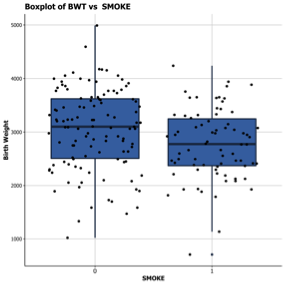
\includegraphics[width=\textwidth]{Images/BWTvsSMOKE.png}
            \label{fig:BWTvsSMOKE}
        \end{subfigure}
        \quad
        \begin{subfigure}[b]{0.3\textwidth}  
            \centering 
            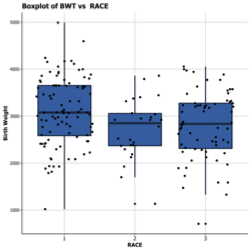
\includegraphics[width=\textwidth]{Images/BWTvsRACE.png}
            \label{fig:BWTvsRACE}
        \end{subfigure}
        
        \hfill
        \medskip
        
        \begin{subfigure}[b]{0.3\textwidth}   
            \centering 
            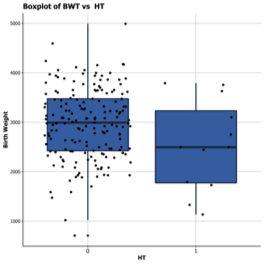
\includegraphics[width=\linewidth]{Images/BWTvsHT.png}
            \label{fig:BWTvsHT}
        \end{subfigure}
        \quad
        \begin{subfigure}[b]{0.3\textwidth}   
            \centering 
            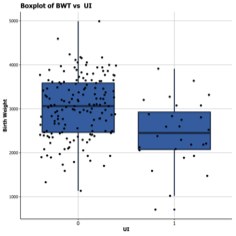
\includegraphics[width=\linewidth]{Images/BWTvsUI.png}
            \label{fig:BWTvsUI}
        \end{subfigure}
        \caption[ The average and standard deviation of critical parameters ]
        {\small Box plots for each of the non-continuous variables against birthweight.} 
        \label{fig:Non-continuous correlation}
    \end{figure}

\textbf{BWT vs RACE:} The mean birth weight for black women and the 'other' group are both slightly lower than for white women (~200 g). These results are consistent with the obstetrical literature.

\textbf{BWT vs SMOKE:} Note that the mean birth weight for smokers is ~2700g and the mean for non-smokers is ~3100g, showing the negative association between smoking and birth weight in our dataset.

\textbf{BWT vs HT:} The mean birth weight for pregnant women with hypertension is lower than the mean birth weight of women with no hypertension history. It is important to note that only a few women in our dataset have a history of hypertension, nonetheless the association is consistent with the literature.

\textbf{BWT vs UI:} Note the 600g difference in mean birth weight between women without UI (3100g) and those with UI (2500g). This is again consistent with the literature and suggests that UI should be strongly considered as a main effect in the candidate models.

\subsection{Interactions Between Sets of Variables}
Drawing from the interactions found in the obstetrical literature, we investigate whether these interactions are also relevant in our dataset. The interactions are visualised int he plots below.

\begin{figure}[!htb]
\minipage{0.32\textwidth}
  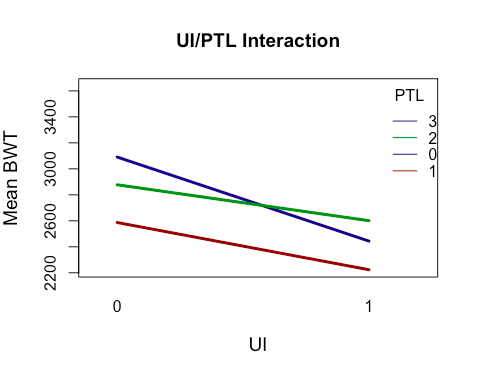
\includegraphics[width=\linewidth]{Images/AGEvsSMOKE.png}
  \caption{}\label{AGEvsSMOKE}
\endminipage\hfill
\minipage{0.32\textwidth}
  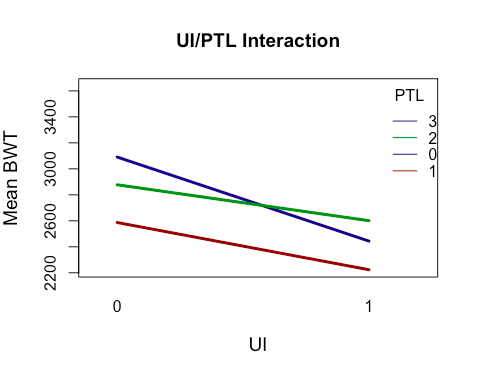
\includegraphics[width=\linewidth]{Images/UIvsPTL.png}
  \caption{}\label{UIvsPTL}
\endminipage\hfill
\minipage{0.32\textwidth}%
  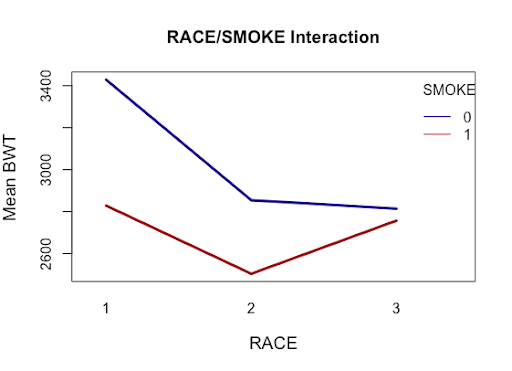
\includegraphics[width=\linewidth]{Images/RACEvsSMOKE.png}
  \caption{}\label{RACEvsSMOKE}
\endminipage
\end{figure}

INSERT INTERACTION EXPLANATION FROM DOCS HERE!!

\section{Question 1}
The four variables which are considered the most clinically important are the AGE, LWT, RACE, and FTV. Using these variables, a model building exercise is carried out to determine the best model to describe the data using the AIC and AIC weights.

\subsection{Model Building} \label{BuildingOne}
There is a trade-off between accuracy and interpretability when deciding on the number of interaction terms to include in these models. The principle of constructing hierarchical models says that if we include an interaction term, the main effect variables should also be included in that interaction. The interaction terms included in the candidate model were the salient interactions determined by the literature review and exploratory analysis. 

First we consider a model with the main effects only:

\begin{equation}
    RACE + FTV + AGE + LWT
\end{equation}

Then a model with all interaction terms:

\begin{equation}
\label{eq:FullModel}
    RACE + FTV + AGE + LWT + LWT/FTV + AGE/FTV
\end{equation}

Then Models with each singular interaction term:

\begin{equation}
    RACE + FTV + AGE + LWT + AGE/FTV
\end{equation}

\begin{equation}
    RACE + FTV + AGE + LWT + LWT/FTV
\end{equation}

The final two candidate models retain $AGE/FTV$ as an interaction term because we have seen that this interaction term is most likely significant through our exploratory data analysis and through model testing. These models examine the effect of adding both LWT and RACE individually as main effects.

\begin{equation}
    RACE + FTV + AGE + LWT + AGE/FTV
\end{equation}

\begin{equation}
    FTV + AGE + LWT + AGE/FTV
\end{equation}

\vspace{0.5cm}
\subsection{Comparing the Models}
The models are evaluated against each other using the Akaike Information Criterion (AIC). The results for the models are shown in \hyperlink{tab:ModelOneComparison}{Table 3}.

\renewcommand{\arraystretch}{1.5}
\begin{table}[!htb]
    \centering
    \begin{tabular}{ |p{8cm}|c|c|c| } 
     \hline
     Model & AIC Score & \Delta Aic & AIC Weight \\
     \hline
     $LOW \thicksim AGE+RACE+FTV+LWT$ & 235.03 & 9.34 & 0.01 \\
     \hline
     $LOW \thicksim AGE+RACE+FTV+LWT+AGE:FTV+LWT:FTV$ & 228.79 & 3.09 & 0.12 \\
     \hline
     $LOW \thicksim AGE+RACE+FTV+LWT+AGE:FTV$ & 227.24 & 1.54 & 0.26 \\
     \hline
     $LOW \thicksim AGE+RACE+FTV+LWT+LWT:FTV$ & 236.64 & 10.94 & 0.00 \\
     \hline
     \rowcolor{blue!25}
     $LOW \thicksim AGE+FTV+LWT+AGE:FTV$ & 225.70 & 0.00 & 0.57 \\
     \hline
     $LOW \thicksim AGE+RACE+FTV+AGE:FTV$ & 231.34 & 5.65 & 0.03 \\
     \hline
    \end{tabular}
    \captionsetup{width=.69\linewidth}
    \caption{Comparison of candidate models using AIC. The best performing model is highlighted.}
    \label{tab:ModelOneComparison}
\end{table}

Based on the AIC weights, we determine that the model 5 is the best model from the list of candidate models. The final model including coefficients is given by:

\begin{equation}
    \mathbb{E}(LOW) = -0.166 + 0.0658 \star AGE + 2.844 \star FTV -0.0155 \star LWT - 0.131 \star Age:FTV 
\end{equation}

A final model was also constructed using the backward elimination procedure. Starting with the full model given by equation \ref{eq:FullModel}, the variable with the highest p-value controlling the type 1 error at $\alpha = 0.1$ was iteratively removed. Both $FTV:LWT$ and $RACE$ were removed using this procedure, resulting in the final model:

\begin{equation}
    \mathbb{E}(LOW) = -0.166 + 0.0658 \star AGE + 2.844 \star FTV -0.0155 \star LWT - 0.131 \star Age:FTV 
\end{equation}

Both the AIC and backward elimination procedures give the same final model.

\subsection{Interpreting the Final Models}

\section{Question Two}

\subsection{Determining Interaction Terms}

\subsection{Model Building} \label{BuildingTwo}

\subsection{Comparing the Models}

\subsection{Interpreting the Final Models}